\documentclass[a4paper,12pt]{article}
\usepackage[T2A]{fontenc}
\usepackage[utf8]{inputenc}
\usepackage[russian]{babel}
\usepackage{amsmath,amssymb}
\usepackage{graphicx}
\usepackage{booktabs}
\usepackage{geometry}
\usepackage{float}
\usepackage{hyperref}
\geometry{left=2cm,right=2cm,top=2cm,bottom=2cm}

\begin{document}

\begin{titlepage}
    \centering
    {\scshape\Large МОСКОВСКИЙ ФИЗИКО-ТЕХНИЧЕСКИЙ ИНСТИТУТ \\
    (НАЦИОНАЛЬНЫЙ ИССЛЕДОВАТЕЛЬСКИЙ УНИВЕРСИТЕТ)\\
    Физтех-школа аэрокосмических технологий}
    \vspace{4cm}
    {\LARGE Отчет о выполнении лабораторной работы 3.3.4}
    \vspace{1cm}
    
    
    {\huge\bf Эффект Холла в полупроводниках}
    \vfill
    \begin{flushright}
        {\LARGE Губарев Никита, Б03-502}
        
        {\LARGE Варлевский Александр, Б03-502}
    \end{flushright}
    \vfill
    \today
\end{titlepage}

\tableofcontents
\newpage

\section{Аннотация}
Цель работы: исследование эффекта Холла в легированном германии, определение постоянной Холла, знака носителей заряда, концентрации, удельной проводимости и подвижности носителей.

\section{Теоретические сведения}
При помещении проводника с током \(I\) в магнитное поле \(B\), перпендикулярное направлению тока, возникает поперечная разность потенциалов (ЭДС Холла):
\begin{equation}
    U_H = R_H \frac{I B}{a},
    \label{eq:hall}
\end{equation}
где \(a\) --- толщина образца в направлении магнитного поля, \(R_H\) --- постоянная Холла. Для полупроводника с носителями одного типа
\begin{equation}
    R_H = \frac{1}{n e},
    \label{eq:RH}
\end{equation}
где \(n\) --- концентрация носителей, \(e = 1{,}602\cdot10^{-19}\)~Кл. Знак \(R_H\) определяется знаком носителей: для электронов \(R_H < 0\), для дырок \(R_H > 0\).

Удельная проводимость \(\sigma\) связана с концентрацией и подвижностью \(\mu\):
\begin{equation}
    \sigma = n e \mu.
    \label{eq:sigma}
\end{equation}
Измерив падение напряжения \(U_{35}\) между контактами 3 и 5 при токе \(I\) в отсутствие магнитного поля, находим проводимость:
\begin{equation}
    \sigma = \frac{I L_{35}}{U_{35} a l},
    \label{eq:cond}
\end{equation}
где \(L_{35}\) --- расстояние между контактами 3 и 5, \(l\) --- ширина образца. Подвижность:
\begin{equation}
    \mu = \frac{\sigma}{n e} = |R_H| \sigma.
    \label{eq:mu}
\end{equation}

\section{Экспериментальная установка и методика}
Схема установки приведена в описании. Магнитное поле создаётся электромагнитом. Индукция \(B\) измерялась двумя независимыми способами.

\paragraph{Датчик Холла ATE-8702.} Прямое измерение \(B\) в зазоре; датчик отградуирован в мТл, показания при \(I_M = 0\) вычитаются как остаточное поле (\(21{,}9\)~мТл).

\paragraph{Милливеберметр (баллистический гальванометр).} Измеряется изменение магнитного потока \(\Delta\Phi\), пронизывающего пробную катушку с произведением площади на число витков
\[
    SN = 75~\text{см}^2 = 7{,}5\cdot10^{-3}~\text{м}^2.
\]
Индукция вычисляется как
\begin{equation}
    B = \frac{\Delta\Phi}{SN}.
    \label{eq:web}
\end{equation}
Для корректной работы милливеберметра в \emph{баллистическом} режиме необходимо выполнение условия
\begin{equation}
    r_{\text{внеш}} \le 5~\text{Ом},
    \label{eq:r}
\end{equation}
где \(r_{\text{внеш}}\) --- суммарное сопротивление измерительной цепи (пробная катушка + подводящие провода + рамка прибора). При \(r_{\text{внеш}} > 5\)~Ом интегрирование ЭДС индукции оказывается неполным, и измеренный поток систематически занижается.

Образец легированного германия подключается к источнику питания; ток \(I\) регулируется реостатом и измеряется миллиамперметром. ЭДС Холла \(U_{34}\) измеряется цифровым вольтметром. Омическое смещение \(U_0\) при \(I_M = 0\) вычитается: \(U_H = U_{34} - U_0\).

Параметры образца: толщина \(a = 1{,}5\)~мм, ширина \(l = 1{,}7\)~мм, расстояние между контактами 3 и 5 \(L_{35} = 3{,}0\)~мм. Ток через образец \(I \le 1\)~мА.

\section{Результаты измерений и обработка}

\subsection{Калибровка электромагнита: сравнение двух методов}
В табл.~\ref{tab:calib} приведены результаты калибровки магнита, полученные двумя независимыми способами.

\begin{table}[H]
    \centering
    \caption{Калибровка электромагнита: сравнение милливеберметра ($SN = 75$~см$^2$) и ATE}
    \label{tab:calib}
    \begin{tabular}{cccccc}
        \toprule
        $I_M$, А & $\Delta\Phi$, мВб & $B_{\text{вебер}}$, мТл & $B_{\text{ATE}}$, мТл & $B_\text{веб}/B_\text{ATE}$ \\
        \midrule
        0    & 0.0 & 0    & 0    & --- \\
        0.24 & 1.1 & 147  & 170.0 & 0.864 \\
        0.48 & 2.3 & 307  & 377.1 & 0.814 \\
        0.75 & 3.4 & 453  & 562.5 & 0.806 \\
        1.00 & 4.4 & 587  & 716.6 & 0.819 \\
        1.25 & 5.3 & 707  & 865.9 & 0.816 \\
        1.50 & 6.0 & 800  & 949.0 & 0.843 \\
        1.77 & 6.4 & 853  & 1015.3 & 0.840 \\
        1.84 & 6.3 & 840  & 1030.0 & 0.816 \\
        \bottomrule
    \end{tabular}
\end{table}

По восьми точкам (без $I_M=0$) отношение \(B_\text{веб}/B_\text{ATE} = 0{,}827 \pm 0{,}018\) остаётся практически постоянным во всём диапазоне поля, то есть значения \(B_\text{вебер}\) систематически ниже \(B_\text{ATE}\) в среднем на \(17\%\). Постоянство отношения указывает на систематическую, а не случайную ошибку.

\paragraph{Интерпретация.} Основная причина расхождения --- несоблюдение условия~\eqref{eq:r}: при \(r_\text{внеш} > 5\)~Ом баллистический режим милливеберметра нарушается, заряд, протекающий через рамку, не успевает полностью проинтегрировать ЭДС индукции, и первый отброс «зайчика» оказывается заниженным. Если эффективное сопротивление цепи превышало \(5\)~Ом в \(1{,}21\) раза, то измеренный поток занижался в \(\sim1{,}21\) раза, что как раз даёт наблюдаемое отношение \(0{,}827\). Альтернативная гипотеза --- неточность номинального \(SN\) (эффективное значение \(\sim 62\)~см$^2$ вместо \(75\)~см$^2$), но она менее вероятна, так как \(SN\) обычно измеряется изготовителем катушки с точностью \(1\text{--}2\%\).

Поскольку датчик ATE-8702 не имеет ограничения по внешнему сопротивлению (электронная схема с высоким входным импедансом), калибровка по ATE принимается как опорная.

\begin{figure}[H]
    \centering
    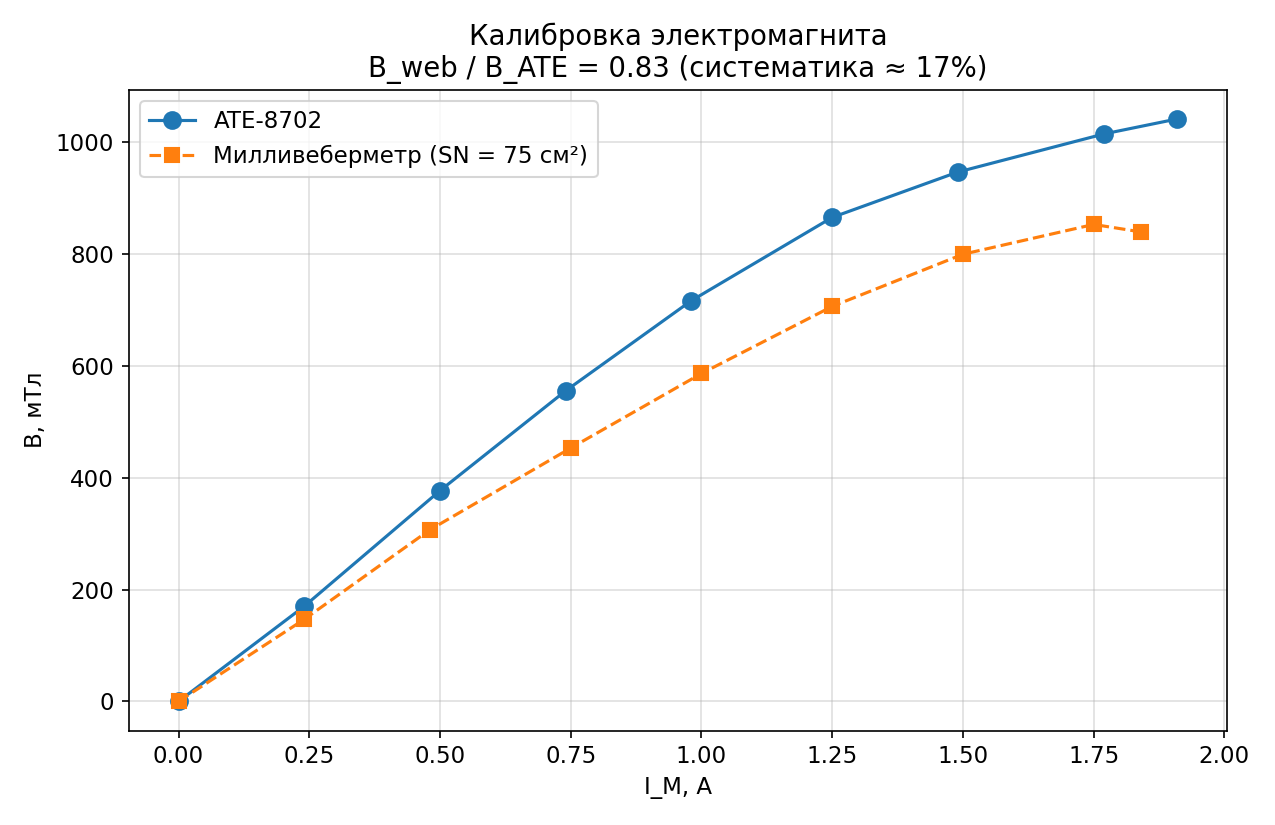
\includegraphics[width=0.82\textwidth]{calib.png}
    \caption{Калибровка электромагнита: ATE (синие кружки) и милливеберметр (оранжевые квадраты). Отношение $B_\text{веб}/B_\text{ATE} = 0{,}827 \pm 0{,}018$ одинаково во всём диапазоне полей, что указывает на систематическую ошибку милливеберметра (вероятно, $r_\text{внеш} > 5$~Ом).}
    \label{fig:calib}
\end{figure}

\subsection{ЭДС Холла}
Для каждого фиксированного тока через образец \(I\) измерялась зависимость \(U_H\) от тока магнита \(I_M\), который пересчитывался в индукцию \(B\) по калибровке ATE. На рис.~\ref{fig:hall} приведены зависимости \(U_H(B)\) для всех 10 токов и для обратного направления поля при \(I = 1\)~мА. Видно, что \(U_H\) линейно зависит от \(B\), а при обращении поля меняет знак. Для положительного направления \(B\) и тока \(I\) (от контакта 1 к 2) напряжение \(U_H\) отрицательно, что соответствует отрицательным носителям заряда (электронам).

\begin{figure}[H]
    \centering
    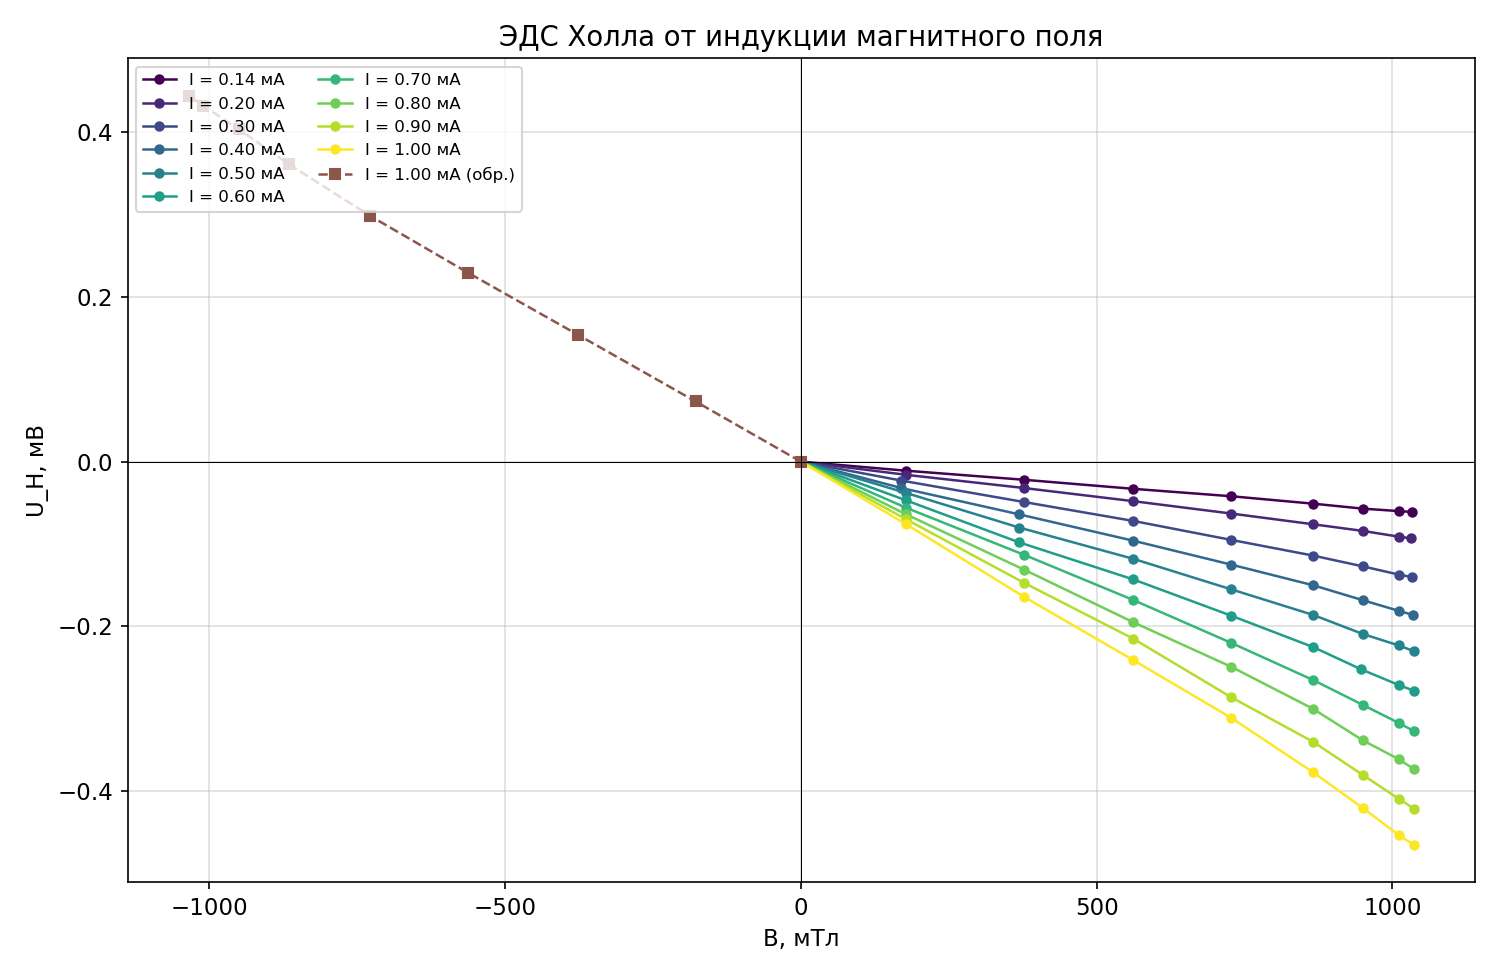
\includegraphics[width=0.92\textwidth]{hall.png}
    \caption{Зависимость ЭДС Холла от индукции магнитного поля для всех токов. Пунктиром показано обратное направление поля при \(I=1\)~мА.}
    \label{fig:hall}
\end{figure}

Для каждого тока проводилась линейная аппроксимация \(U_H = \alpha B + \beta\). Наклон \(\alpha = dU_H/dB\) связан с постоянной Холла:
\begin{equation}
    R_H = \frac{\alpha\, a}{I}.
\end{equation}
Результаты расчёта \(R_H\) сведены в табл.~\ref{tab:RH}. Погрешности в таблице — статистические (из МНК); полные погрешности с учётом неточности \(a\) и \(B\) приведены ниже.

\begin{table}[H]
    \centering
    \caption{Наклоны \(\alpha\) и постоянная Холла \(R_H\). Точка $I = 0{,}14$~мА --- выброс, исключена из усреднения.}
    \label{tab:RH}
    \begin{tabular}{cccc}
        \toprule
        $I$, мА & $\alpha = dU_H/dB$, мВ/Тл & $R_H$, $10^{-3}$~м$^3$/Кл (стат.) & Примечание \\
        \midrule
        0.14 & $-0{,}0592$ & $-0{,}634 \pm 0{,}006$ & выброс \\
        0.20 & $-0{,}0897$ & $-0{,}673 \pm 0{,}009$ & \\
        0.30 & $-0{,}1349$ & $-0{,}674 \pm 0{,}009$ & \\
        0.40 & $-0{,}1775$ & $-0{,}666 \pm 0{,}010$ & \\
        0.50 & $-0{,}2207$ & $-0{,}662 \pm 0{,}008$ & \\
        0.60 & $-0{,}2665$ & $-0{,}666 \pm 0{,}009$ & \\
        0.70 & $-0{,}3132$ & $-0{,}671 \pm 0{,}009$ & \\
        0.80 & $-0{,}3562$ & $-0{,}668 \pm 0{,}009$ & \\
        0.90 & $-0{,}4042$ & $-0{,}674 \pm 0{,}008$ & \\
        1.00 & $-0{,}4467$ & $-0{,}670 \pm 0{,}008$ & \\
        \bottomrule
    \end{tabular}
\end{table}

Точка \(I = 0{,}14\)~мА даёт \(R_H\), отклоняющееся от остальных на \(6\%\), что превышает её статистическую погрешность. При малом токе сказываются остаточные наводки и дрейф нуля вольтметра, поэтому она исключена.

Среднее значение постоянной Холла (по 9 точкам, взвешенное по обратным дисперсиям):
\[
    \langle R_H \rangle = -(0{,}6694 \pm 0{,}0029_{\text{стат}})\cdot 10^{-3}~\text{м}^3/\text{Кл}.
\]
С учётом систематики от неточности \(a\) (\(\delta a/a \approx 6{,}7\%\)) полная погрешность:
\[
    \langle R_H \rangle = -(0{,}669 \pm 0{,}045)\cdot 10^{-3}~\text{м}^3/\text{Кл}.
\]
Знак «минус» указывает на электронный тип проводимости (n-тип).

\begin{figure}[H]
    \centering
    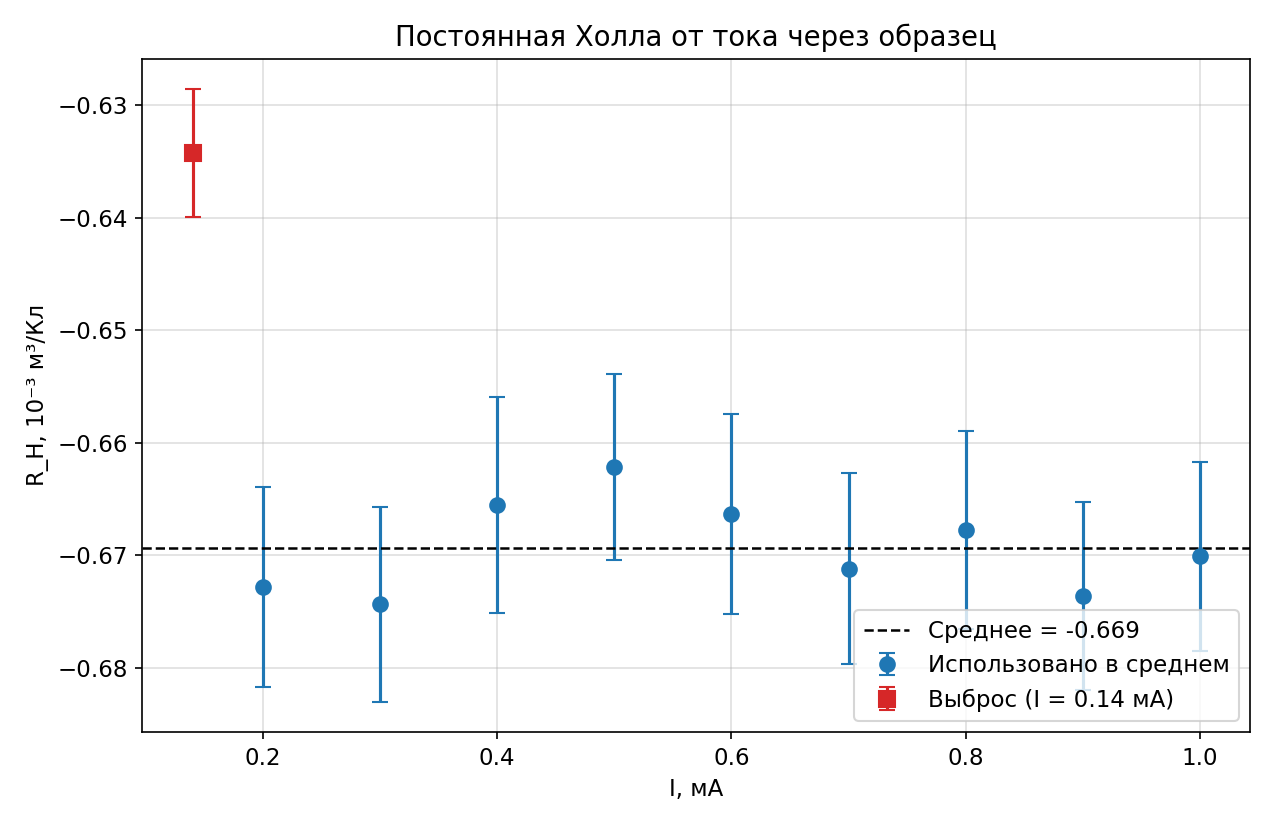
\includegraphics[width=0.82\textwidth]{Rh.png}
    \caption{Постоянная Холла от тока. Синие точки --- использованы в среднем, красный квадрат --- выброс $I = 0{,}14$~мА.}
    \label{fig:Rh}
\end{figure}

\subsection{Концентрация и подвижность}
Концентрация носителей:
\[
    n = \frac{1}{|R_H| e} = \frac{1}{0{,}6694\cdot 10^{-3} \cdot 1{,}602\cdot 10^{-19}} \approx 9{,}33\cdot 10^{21}~\text{м}^{-3} = 9{,}33\cdot 10^{15}~\text{см}^{-3}.
\]
Статистическая погрешность \(n\):
\[
    \delta n_{\text{стат}} = n\cdot\frac{0{,}0029}{0{,}6694} \approx 0{,}04\cdot 10^{21}~\text{м}^{-3}.
\]
С учётом систематики (та же \(6{,}7\%\)) полная погрешность \(\delta n \approx 0{,}63\cdot 10^{21}\)~м$^{-3}$.

Удельная проводимость по формуле~\eqref{eq:cond} с \(U_{35} = 1{,}839\)~мВ при \(I = 1\)~мА:
\[
    \sigma = \frac{1\cdot10^{-3}\cdot 3\cdot10^{-3}}{1{,}839\cdot10^{-3} \cdot 1{,}5\cdot10^{-3} \cdot 1{,}7\cdot10^{-3}} \approx 6{,}40\cdot10^{2}~\text{См/м}.
\]
Погрешность \(\sigma\) (с учётом \(\delta a/a\), \(\delta l/l\), \(\delta L_{35}/L_{35}\), \(\delta I/I\), \(\delta U_{35}/U_{35}\)):
\[
    \delta\sigma = 0{,}61\cdot 10^{2}~\text{См/м}.
\]

Подвижность:
\[
    \mu = |R_H| \sigma \approx 0{,}6694\cdot10^{-3} \cdot 6{,}397\cdot10^{2} \approx 0{,}428~\text{м}^2/(\text{В}\cdot\text{с}) = 4{,}28\cdot 10^{3}~\text{см}^2/(\text{В}\cdot\text{с}).
\]
Погрешность \(\mu\) (консервативная оценка, с учётом неточности \(\sigma\)):
\[
    \delta\mu \approx 0{,}041~\text{м}^2/(\text{В}\cdot\text{с}) = 4{,}10\cdot 10^{2}~\text{см}^2/(\text{В}\cdot\text{с}).
\]

\section{Сводная таблица результатов}
\begin{table}[H]
    \centering
    \caption{Итоговые параметры образца (в скобках --- статистическая погрешность, без скобок --- полная)}
    \begin{tabular}{lcc}
        \toprule
        Величина & Значение & Погрешность \\
        \midrule
        \(R_H\) & \(-0{,}6694\cdot 10^{-3}\)~м$^3$/Кл & \(0{,}0029_{\text{стат}}\) ($0{,}045$ полн.) $\cdot 10^{-3}$~м$^3$/Кл \\
        Тип носителей & электроны (n-тип) & \\
        \(n\) & \(9{,}33\cdot 10^{21}\)~м$^{-3}$ & \(0{,}04_{\text{стат}}\) ($0{,}63$ полн.) $\cdot 10^{21}$~м$^{-3}$ \\
        \(\sigma\) & \(6{,}40\cdot 10^{2}\)~См/м & \(0{,}61\cdot 10^{2}\)~См/м \\
        \(\mu\) & \(4{,}28\cdot 10^{3}\)~см$^2$/(В$\cdot$с) & \(0{,}41\cdot 10^{3}\)~см$^2$/(В$\cdot$с) \\
        \bottomrule
    \end{tabular}
\end{table}

\section{Оценка погрешностей}
Основные источники:
\begin{itemize}
    \item \(U_H\) (\(\pm1\)~мкВ): \(\delta\alpha/\alpha \approx 2\text{--}3\%\);
    \item калибровка ATE и интерполяция \(B\): \(\delta B/B \approx 2\%\);
    \item геометрические размеры: \(\delta a/a \approx 6{,}7\%\), \(\delta l/l \approx 5{,}9\%\), \(\delta L_{35}/L_{35} \approx 3{,}3\%\);
    \item ток через образец: \(\delta I/I \approx 1\%\);
    \item \(U_{35}\): \(\delta U_{35}/U_{35} \approx 0{,}05\%\).
\end{itemize}
Суммарные относительные погрешности:
\[
    \frac{\delta R_H}{R_H} \approx 6{,}7\%\ (\text{геометрия}),\quad
    \frac{\delta n}{n} \approx 6{,}7\%,\quad
    \frac{\delta\sigma}{\sigma} \approx 9{,}6\%,\quad
    \frac{\delta\mu}{\mu} \approx 9{,}6\%.
\]
Доминирующий вклад --- неточность геометрических размеров образца. Заметим, что в формуле \(\mu = |R_H|\sigma = \alpha L_{35}/(U_{35} l)\) толщина \(a\) сокращается, поэтому \(\mu\) в действительности не зависит от \(a\); приведённая оценка \(\delta\mu/\mu \approx 9{,}6\%\) является консервативной (сверху).

\section{Выводы}
1. Исследован эффект Холла в легированном германии. Измерена зависимость ЭДС Холла от магнитного поля при 10 токах через образец и при обратном направлении поля.
2. Проведено сравнение двух методов калибровки магнитного поля: датчик Холла ATE-8702 и милливеберметр (\(SN = 75\)~см$^2$). Обнаружено систематическое расхождение \(17\%\), при котором \(B_\text{веб}/B_\text{ATE} = 0{,}827 \pm 0{,}018\) постоянно во всём диапазоне полей. Наиболее вероятная причина --- несоблюдение условия \(r_\text{внеш} \le 5\)~Ом для баллистического режима милливеберметра, приводящее к неполному интегрированию ЭДС индукции. Для анализа использована калибровка ATE как опорная.
3. Из расчёта \(R_H\) исключена точка \(I = 0{,}14\)~мА, дающая отклонение \(\sim6\%\) (влияние наводок и дрейфа нуля при малом токе).
4. Определена постоянная Холла \(R_H = -(0{,}669 \pm 0{,}045)\cdot 10^{-3}\)~м$^3$/Кл (полная погрешность). Отрицательный знак указывает на электронный тип проводимости (n-тип).
5. Рассчитаны концентрация носителей \(n = (9{,}33 \pm 0{,}63)\cdot 10^{21}\)~м$^{-3} = (9{,}33 \pm 0{,}63)\cdot 10^{15}$~см$^{-3}$, удельная проводимость \(\sigma = (6{,}40 \pm 0{,}61)\cdot 10^{2}\)~См/м и подвижность \(\mu = (4{,}28 \pm 0{,}41)\cdot 10^{3}\)~см$^2$/(В$\cdot$с).
6. Полученные значения соответствуют типичным параметрам легированного германия (для Ge \(\mu_e \approx 3900\)~см$^2$/(В$\cdot$с)). Расхождение с табличными данными объясняется главным образом неточностью геометрических размеров образца.

\appendix
\section{Графики}
\begin{figure}[H]\centering
    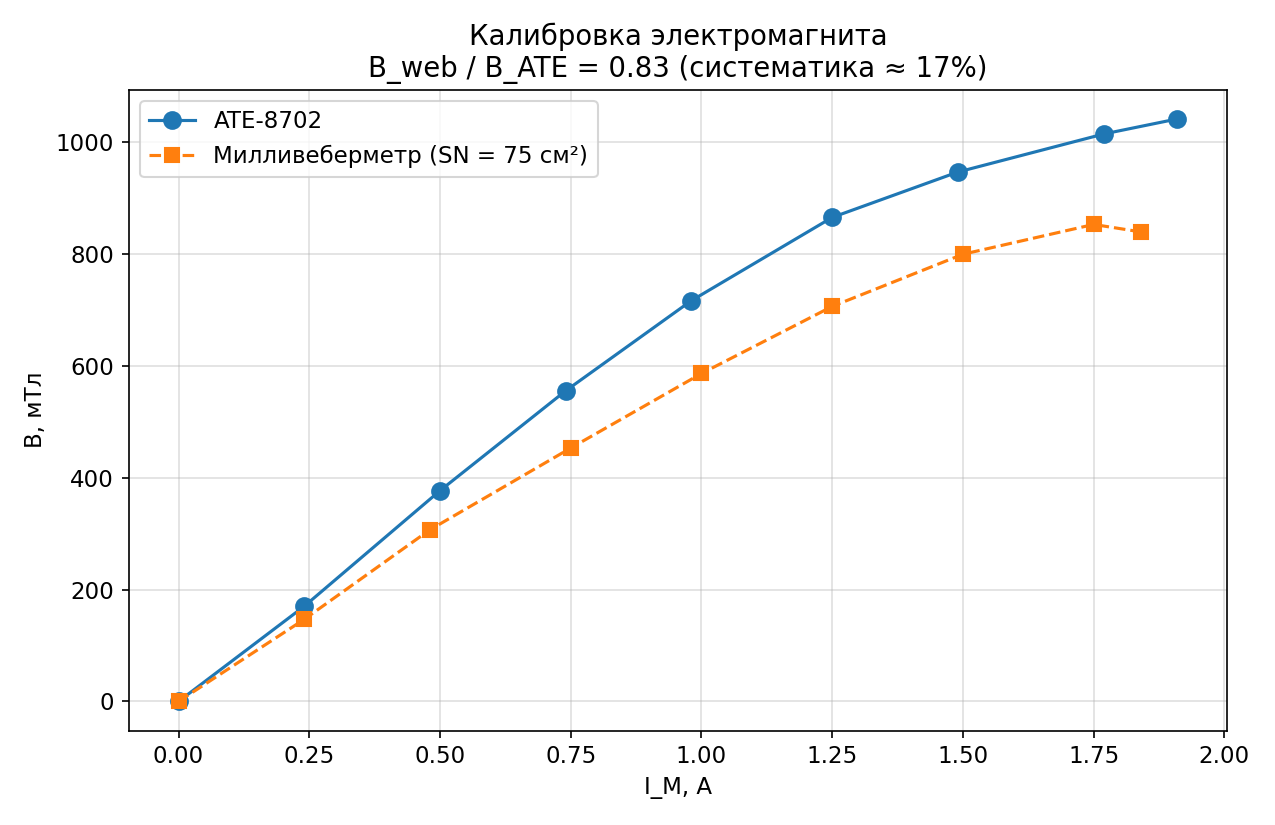
\includegraphics[width=0.82\textwidth]{calib.png}
    \caption{Калибровка электромагнита: ATE vs милливеберметр}
\end{figure}
\begin{figure}[H]\centering
    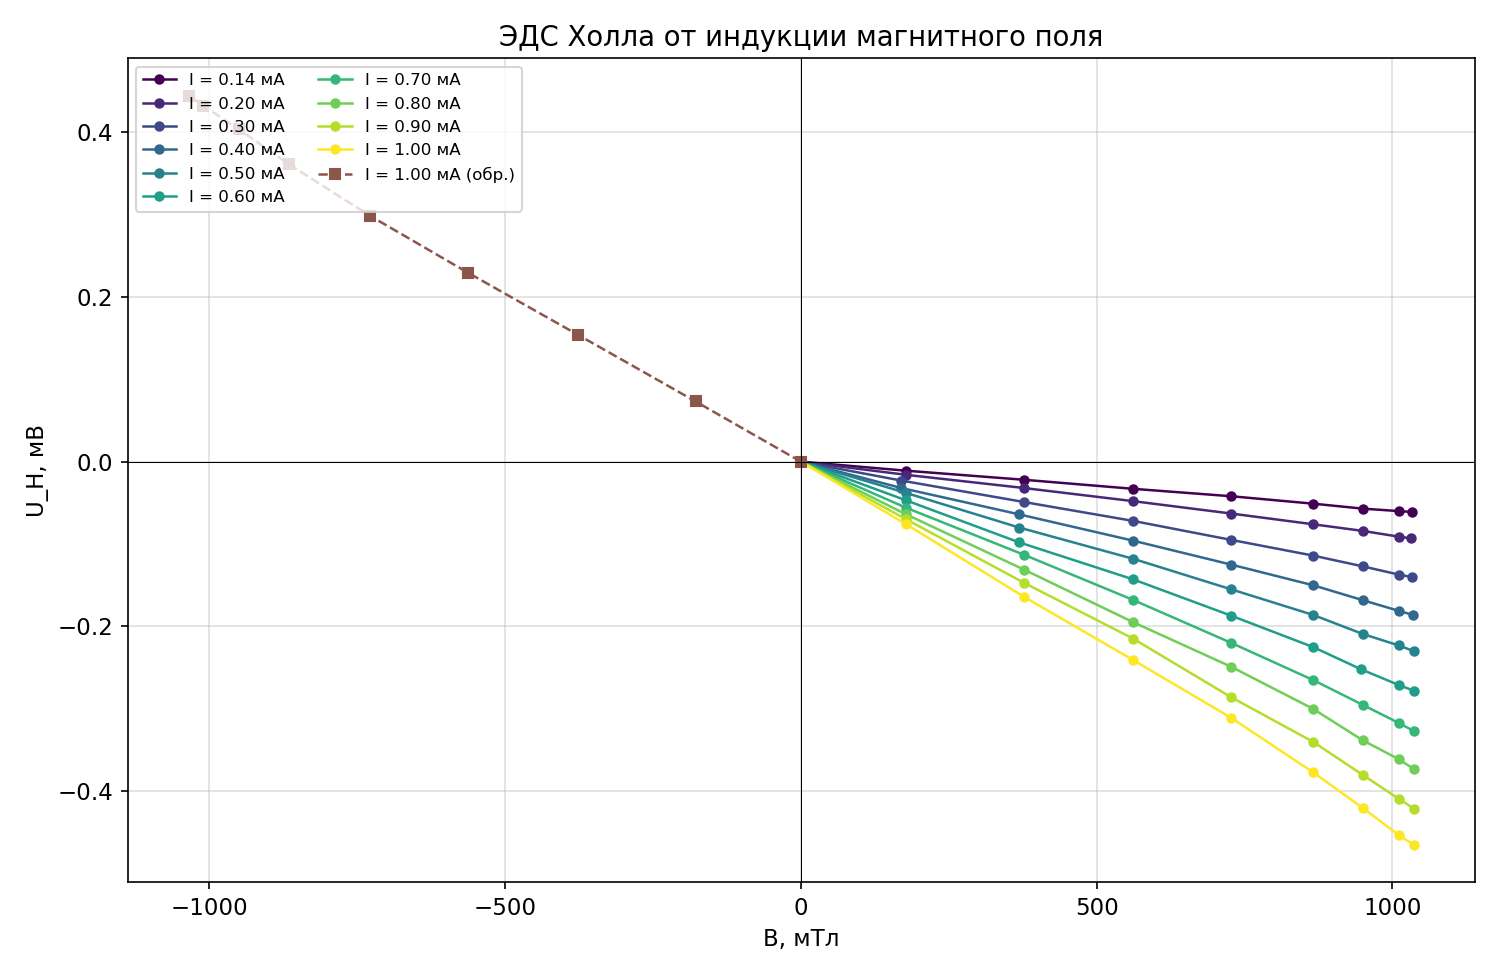
\includegraphics[width=0.92\textwidth]{hall.png}
    \caption{ЭДС Холла от индукции поля для всех токов}
\end{figure}
\begin{figure}[H]\centering
    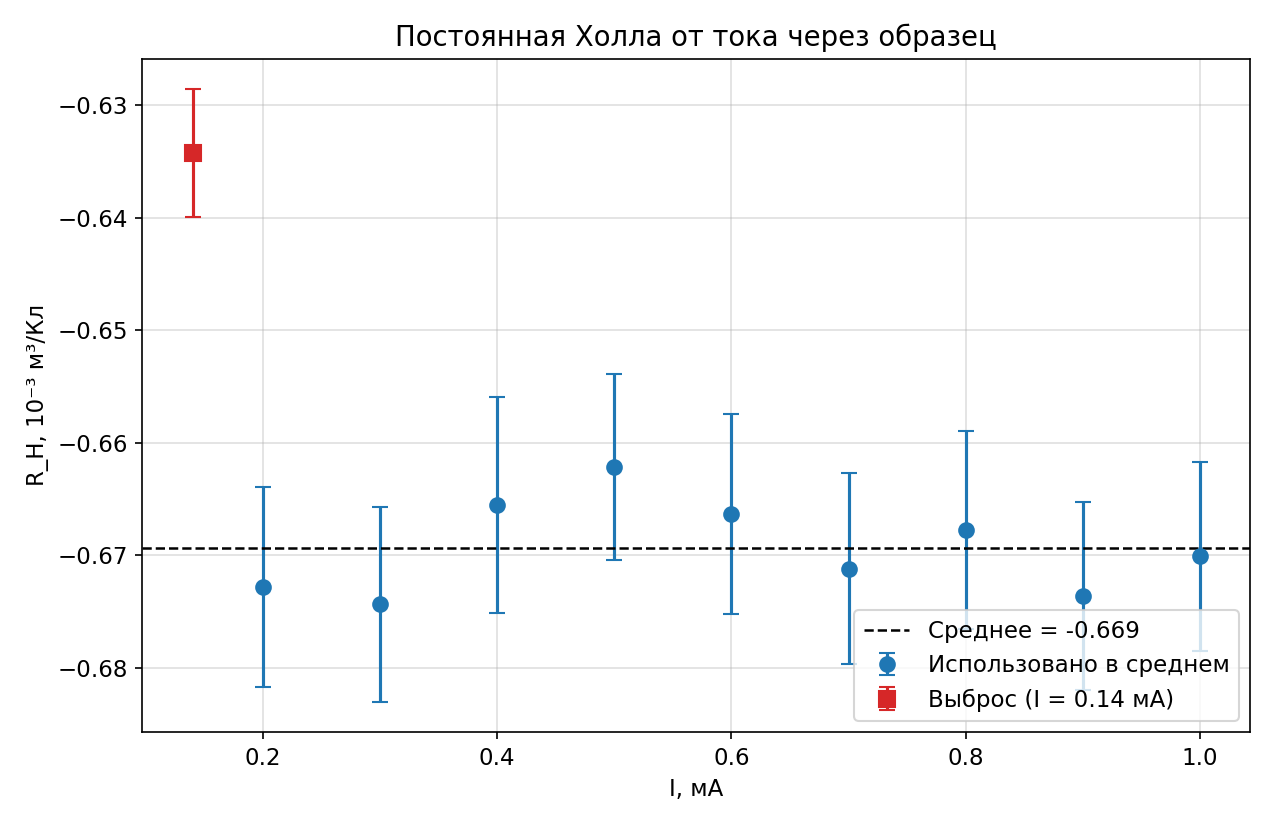
\includegraphics[width=0.82\textwidth]{Rh.png}
    \caption{Постоянная Холла от тока через образец}
\end{figure}

\end{document}
